\documentclass[class=article, crop=false]{standalone}

\usepackage{./resources/style}
\usepackage{./resources/referencing}


\title{Deriving the Normal Distribution}
\author{Ryan Greenup}
\date{Autumn 2020}

\begin{document}
\hypertarget{power-series-and-uniform-continuity}{%
\section{Power Series and Uniform
Continuity}\label{power-series-and-uniform-continuity}}

\hypertarget{power-series}{%
\subsection{Power Series}\label{power-series}}

\hypertarget{convergence}{%
\subsubsection{Convergence}\label{convergence}}

A sequence \(x=(x_n)\) converges if:

\begin{align*}
\forall \varepsilon > 0, \quad \exists N:&
\ \\
&n \geq N \implies |x_n - x | < \varepsilon
\end{align*}

and it is hence expressed:

\[
\lim(x_n) = x
\]

A series is generated by a sequence,

If \((a_n)\) is a sequence, the series is \((S_n)\):

\begin{align*}
S_1 &= a_1 \\
s_2&= S_1 +  a_2 \\
S_3&= S_2 +  a_3\\
S_4&= S_3+ a_4\\
\cdots
\end{align*}

The series is convergent if:

\begin{align*}
  \forall \varepsilon > 0, \exists N:&\\
&  n \geq N \ \implies    \left| S_n - L \right|  < \varepsilon
\end{align*}

The series is absolutely convergent if $\left\lvert S_n \right\rvert$ is convergent.

The notation for series used is:

\begin{align*}
\sum^{\infty}_{n=1} \left[ \left( a_n \right)  \right] = \sum \left( a_n \right) = \lim_{}\left[ S_n \right]
\end{align*}

Be mindful that this notation is used ambiguously to represent both:

\begin{itemize}
\item
  The infinite Series
\item
  The limit value of the series.
\end{itemize}

In practice however the ambiguity is a non-issue because context will
discern the difference.

\hypertarget{sequences-of-functionstbook}{%
\subsubsection[Sequences of Functions]{\texorpdfstring{Sequences of
Functions\footnote{This is in the Bartle and Sherbert Textbook at
  Chapter {[}8.1.7{]} p.~246}}{Sequences of Functions}}\label{sequences-of-functionstbook}}

We can have sequences of real numbers, and similarly we can have
sequences of functions.

Sequences of functions can converge in two ways:

\begin{itemize}
\item
  Pointwise
\item
  uniformly
\end{itemize}

Uniform convergence is important because it preserves term properties to
the limit function which will be seen.

\hypertarget{define-a-sequence-of-functions}{%
\paragraph{Define a sequence of
functions:}\label{define-a-sequence-of-functions}}

Let $A \subseteq \mathbb{R} , n \in \mathbb{N}$ and take some
function \(f\) :


\begin{align*}
f_n: A     \rightarrow \mathbb{R}
\end{align*}

 It is said that $\left( f\_n \right)$ is a sequence of functions
on \(A\) to $\mathbb{R}$.

For every \(x \in A\) there will be a sequence of real numbers:


\begin{align*}
f_n\left( x \right)
\end{align*}

 For some values of \(x\), the sequence may converge, for others it
may not.

\begin{itemize}
\item
  The point of convergence is
  \( \lim\_\{\}\left[ f_n\left( x_n \right)  \right] \) which depends on
  the choice of \(x\).
\item
  Thus we could Create a set of all \(x \in A\) forwhich
  \(\left( f_n\left( x \right) \right)\) converges.

  \begin{itemize}
  \item
    This set would be a domain for a function $f\left( x \right)$
    that would act as the limit of the sequence \(\left( f\_n\left( x
    \right) \right) \).
  \end{itemize}
\end{itemize}

\hypertarget{pointwise-convergence}{%
\paragraph{Pointwise Convergence}\label{pointwise-convergence}}

Take some function:

  \begin{align*}
  f: A_0     \rightarrow  \mathbb{R} \qquad \left( A_0 \subseteq A \subseteq \mathbb{R}  \right)
  \end{align*}

We say that the sequence is pointwise convergent if,

\begin{itemize}
\item
  for every \(x \in A_0\)

  \begin{itemize}
  \item
    The sequence \(\left( f\_n\left( x \right) \right) \) converges to
    \(f\left( x \right) \).
  \end{itemize}

  e.g.~\(\ \ \) consider \(g_n\left( x \right) : = x^n\);

  \begin{align*}
    \left( g_n\left( x \right)  \right) = \left( x, x^2, x^3, x^4 \cdots \right)
  \end{align*}
   If \(- 1 < x < 1 \quad\), then $x$ is a fraction or zero so:
  \begin{align*}
    \left( x, x^2, x^3, x^4 \cdots 0 \right) \qquad \text{ Converges to 0}
  \end{align*}

  if \(x = 1\), then:

  \begin{align*}
    \left( x, x^2, x^3 \cdots \right) = \left( 1, 1^2, 1^3, \cdots 1 \right)  \qquad \text{Converges to 1}
    \end{align*}

   if \(x= -1\), then:

  \begin{align*}
    \left( x, x^2, x^3, \cdots \right) = \left( 1, - 1, 1, - 1, \cdots \pm 1 \right) \qquad \text{Divergent}
  \end{align*}


  if \(\left\lvert x \right\rvert > 1\), then:

  \begin{align*}
    \left( x, x^2, x^3, \cdots \infty \right) \qquad \text{Divergent}
  \end{align*}

  So \(\lim\_\{\}\left[ g_n\left( x \right)  \right]\) on the set
  \(\left(- 1, 1\right] \) where:

  \begin{align*}
  g\left( x \right) =
  \begin{cases}
    0, \qquad \text{for} \enspace \left( - 1<x<1 \right) \\
    1,\qquad \text{for} \enspace \left( x = 1 \right)
  \end{cases}
  \end{align*}

\end{itemize}

\hypertarget{definition}{%
\paragraph{Definition}\label{definition}}

An alternative, but equivalent definition for pointwise convergence is:

\begin{align}
  \forall \varepsilon>0, \enspace \forall &x \in A_0, \enspace \exists N:\\
  \ \\
&n \geq N  \implies       \left| f_n\left( x \right)  -  f\left( x \right)  \right| < \varepsilon
\end{align}

Where \(N\) is a function of \(x\) and \(\varepsilon\), i.e.:

\begin{itemize}
\item
  \(N = N\left( \varepsilon, x \right)\).
\end{itemize}

\#\#\#Definition of Power Series A power series is a series of the form:

\begin{align}
  \sum^{\infty}_{n= 0} \left[ c_nx^n \right] = c_0+ c_1x+ c_2x^2+ c_3x^3 + \cdots
\end{align}

More generally a series will be of the form:

\begin{align}
  \sum^{\infty}_{n= 0} \left[ c_n \left( x- a \right) ^n \right] = c_0 +  c_1\left( x- a \right) + c_2\left( x- a \right) ^2 +  \cdots
\end{align}
 \#\#\#\# Convergence of Power Series For any given power series of
the form \( \sum\{\infty\}\_\{n= 0\}
\left[ c_n \left( x- a \right) ^n \right]\) there are only three
possibilities:

\begin{enumerate}
\def\labelenumi{\arabic{enumi}.}
\item
  The series converges only when \(x = a\)
\item
  The series converges for all x.
\item
  There is a positive number \(R\) such that the series converges if \(
  \left\lvert x- a \right\rvert \textless{} R\) and diverges if
  \( \left\lvert x - a \right\rvert \textgreater{} R\).
\end{enumerate}

\hypertarget{why-power-series}{%
\paragraph{Why power Series}\label{why-power-series}}

The whole idea of power series is representing a known function as an
infinite series, this is useful for integrating functions that don't
have elementary antiderivatives.

Take for example the geometric series:
\begin{align}
  \sum^{\infty}_{n= 0} \left[ ax^n \right] &= \frac{a}{1 - x}\\
  & \implies  f\left( x \right) = \frac{a}{1-x} = \sum^{\infty}_{n= 0} \left[ ax^n \right]
\end{align}

\hypertarget{example}{%
\subparagraph{Example}\label{example}}

Find a power series representation for
\(f\left( x \right) = \frac{x^3}{x + 2}\)

\begin{align}
  \frac{1}{2 +  x} =  \frac{1}{2\left( 1+ \frac{x}{2} \right) }\\
  &=  \frac{1}{2\left( 1 - \left( - \frac{x}{2} \right)  \right) }\\
  &= \frac{1}{2} \cdot \sum^{\infty}_{n= 0} \left[ - \frac{x}{2} \right] ^n\\
  &= \sum^{\infty}_{n= 0} \left[ \frac{\left( - 1 \right) ^n}{2^{n +  1}} \cdot  x^n \right] \\
  \implies   \frac{x^3}{2 +  x } &=  \sum^{\infty}_{n= 0} \left[ \frac{\left( -1  \right) ^n}{2^{n+ 1}}\cdot x^{n+ 3} \right]
\end{align}

 because this is a geometric series, it converges when:
\begin{align}
  \left| - \frac{x}{2} \right| &< 1\\
  & \implies  x \in \left( - 2, 2 \right)\\
 & \tiny{  \text{ This is known as the radius of convergence $\left( R= 2 \right) $} }
\end{align}

So from this we could show something like:
\begin{alignat}{5}
  f\left( x \right) = &\frac{x^3}{2+ x} &=& &\sum^{\infty}_{n= 0} &\left[ \frac{\left( - 1 \right) ^n}{2^{n+ 1}}\cdot x^{n+ 3} \right]&\\
  \int^{}_{} &\frac{x^3}{2+ x}  \operatorname{d}x \enspace  &=& \enspace C + &\sum^{\infty}_{n= 0} &\left[ \frac{\left( - 1 \right) ^n}{2^{n+ 1}} \cdot  \frac{x^{n+ 4}}{n+ 4} \right]   &
\end{alignat}

The important part with all of this is that it works with Taylor
Series.\footnote{\href{https://www.dropbox.com/s/z4t4aebk15iyuc8/Proof\%20of\%20Taylor\%20series.pdf?dl=0}{Refer
  to Ch. 58, p.~190 of \emph{Churchill's Complex Variables} 9thEd.}}

\hypertarget{convergence-of-power-series}{%
\subsubsection{Convergence of Power
Series}\label{convergence-of-power-series}}

if \(\sum\{\infty\}\_\{n= 0\}
\left[ a_n\cdot \left( z- z_0 \right)^n  \right] \) is convergent for
some \(z= \alpha\) then, * It will converge absolutely for all values of
\( \left\rvert z- z\_0 \right\rvert > \left\rvert
z- \alpha \right\rvert \)

\hypertarget{uniform-convergence-of-power-series}{%
\subsubsection{Uniform Convergence of Power
Series}\label{uniform-convergence-of-power-series}}

if \(\sum\{\infty\}\_\{n= 0\}
\left[ a_n\cdot \left( z- z_0 \right) ^n \right] \) converges when
\(z = \alpha\) but \(\left( \alpha \neq z_0 \right)\)  : * Then the
series converges uniformly in any open-neighbourhood:

  \begin{align*}
        \left| z- z_0 \right| \leq r&\\
&        \text{Where} \enspace r =     \left| z_0 - \alpha \right|
  \end{align*}

\begin{itemize}
\item
  The sum of the series represents an analytic function, i.e.:
  \begin{align*}
  f\left( z \right) = \sum^{\infty}_{n= 0}   \left[ a_n\cdot \left( z- z_0 \right) ^n \right]
  \end{align*}
 Such that \(f\left( z \right) \) is an analytic function that can
  also be represented by the power series
\end{itemize}

\hypertarget{circle-of-convergence}{%
\subsubsection{Circle of Convergence}\label{circle-of-convergence}}

\(\sum\{\infty\}\_\{n= 0\}
\left[ a_n\cdot \left( z- \alpha \right) ^n \right] \) is convergent
only for \( \left\lvert{} z- \alpha \right\rvert{} \textless R\) :

\begin{itemize}
\item
  if \(R= 0\), the series is only convergent for \(z= \alpha\)
\item
  if \(r = \infty\), the series is convergent \(\forall z\in \mathbb{C}
  \)
\item
  if \(R \in \mathbb{R} ^+\), the series is convergent on some open disc
  centred at \(\alpha\) of radius R.
\end{itemize}

\hypertarget{taylor-seriestsrs3}{%
\subsubsection[Taylor Series]{\texorpdfstring{Taylor
Series\footnote{\href{https://www.youtube.com/watch?v=3d6DsjIBzJ4}{\emph{3Blue1Brown}
  does a nice video on this} If a function is analytic at \(\alpha\) and
  in an open disc \( \left\lvert{} z- \alpha \right\rvert{}
  \textless R\), there will always be a power series representation of
  \(f\left( z \right) \) :}}{Taylor Series}}\label{taylor-seriestsrs3}}

\begin{align*}
  f\left( z \right) =  \sum^{\infty}_{n= 0}   \left[ a_n\cdot \left( z- \alpha \right) ^n \right] , \qquad     \left| z- z_0 \right| < r&\\
  \text{where:}\enspace a_n &= \frac{f^{\left( n \right) }\left( z_0 \right) }{n!}
\end{align*}
 This can be shown using the \emph{Cauchy Integral Formula}, however a
clearer justification is:

\begin{itemize}
\item
  If a function a power series representation for a function exists:
\end{itemize}

\begin{align*}
  f\left( z \right) &= \sum^{\infty}_{n= 0}   \left[ c_n\cdot \left( z- \alpha \right) ^n \right] \qquad {\tiny \text{$C_n$ and $\alpha$ are complex constants}}\\
  &= c_0 +  c_1\left( z- \alpha \right) + c_2\left( z- \alpha \right) ^2 \cdots\\
  \implies   f \left( \alpha \right) &= c_0\times 0^0 +  c_1\times 0 + 0 + \cdots \\
  &= c_0\\
\end{align*}
 Consider the first derivative:
\begin{align*}
f'\left( z \right) &= c_1 + 2\cdot c_2\left( z- \alpha \right) + 3\cdot c_2\cdot \left( z\alpha \right) ^2\cdots\\
 \implies  f'\left( \alpha \right) &= c_1
\end{align*}

Consider the second derivative:
\begin{align*}
  f''\left( z \right) &= 2\cdot c_2+ 3\times 2\cdot \left( z- \alpha \right) + 4\times 3\times 2\cdot \left( z- \alpha \right) ^2+  \cdots\\
  &= 2!c_2 +  3!\left( z- \alpha \right) + 4!\cdot \left( z- \alpha \right) ^2+  \cdots\\
  f''\left( \alpha \right) &= 2c_2
\end{align*}

By this logic the nth derivative will be:

\begin{align*}
  f^{\left( n \right) }&= n!\cdot c_n\\
  \implies  c_n&= \frac{f^{\left( n \right) }\left( \alpha \right) }{n!}
\end{align*}

We will always be able to find \(c_n\) where \(f\left( z \right) \) is
analytic and clearly the power series will be convergent (i.e.~to
\(f\left( z \right) \)) on a radius of convergence where \(f\left( z
\right) \) is analytic, so:

\begin{align*}
  f\left( z \right) &= \sum^{\infty}_{n= 0}   \left[ \frac{f^{\left( n \right) }\left( \alpha \right) }{n!} \times \left( z- \alpha \right)  \right] , \qquad    & \left| z- z_0 \right| <R \\
  &&{\tiny \text{$R$ is the radius of the open disc of analyticity}}
\end{align*}

\subsubsection{The Cauchy Hadamard Theorem If we have a power series:}

\begin{align*}
\sum^{\infty}_{n= 0}   \left[ a_n\cdot \left( z- z_0 \right) ^n \right]
\end{align*}

Then we can find the radius of convergence:

\begin{align*}
  l&= \limsup{    \left[ \left| a_n \right| ^{\frac{1}{n}} \right] }\\
  \ \\
  & \implies  R = \frac{1}{l}
\end{align*}

Further if * \( \left\lvert{} a\_n \right\rvert{} \neq\_0\) and
\(\lim_{}\left[ \left| \frac{a_{n+ 1}}{a_n} \right| \right] = R\) Then:
*
\(\lim_{}\left[ \left| a_n \right| ^{\frac{1}{n}} \right] = \lim_{}\left[ \left| \frac{a_{n+ 1}}{a_n} \right| \right] = R\)

Generally the \(n^{\text{th}}\) root test is more powerful than the
ratio test, however the ratio test is the only test that can deal with
factorials\footnote{\href{http://tutorial.math.lamar.edu/Classes/CalcII/SeriesStrategy.aspx}{How
  to choose a test by pauls Online Notes}}, so it is important to have
it in our toolbox.

\hypertarget{uniform-continuity}{%
\subsection{Uniform Continuity}\label{uniform-continuity}}

\hypertarget{what-is-uniform-continuity}{%
\subsubsection{What is uniform
continuity}\label{what-is-uniform-continuity}}

Imagine the function \(y= \frac{1}{x}\) and consider the interval
\(\left( 0,\infty \right) \), * Consider the limit value of 2 (e.g.~the
line \(y= 2\) )

\begin{figure}
\centering
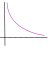
\includegraphics{"./media/ComplexSeries/drawing.png"}
\caption{drawing}
\end{figure}

If I choose some \(\varepsilon\) value, there is always a corresponding
\(\delta\)-value, this \(\delta\)-value will depend on the
\(\varepsilon\)-value:

\begin{figure}
\centering
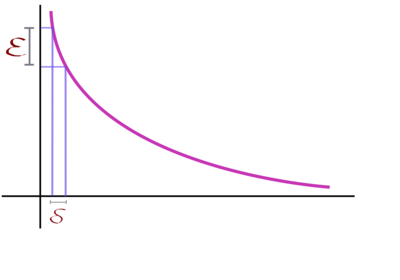
\includegraphics{./media/ComplexSeries/drawing2.png}
\caption{drawing2}
\end{figure}

so the function \(f\left( x \right) = \frac{1}{x}\) is continuous
because: * \(\varepsilon\) can be chosen anywhere * Any \(\varepsilon\)
value will have a corresponding \(\delta\) value.

The function would be uniformly continuous, if: * \(\varepsilon\) can be
chosen anywhere * The Corresponding \(\delta\) value will exist AND not
change size wherever \(\varepsilon\) is chosen.

So in this case the function is not uniformly continuous, because if I
move \(\varepsilon\) down, \(\delta\) would have to get larger, so it IS
NOT uniformly continuous:

\begin{figure}
\centering
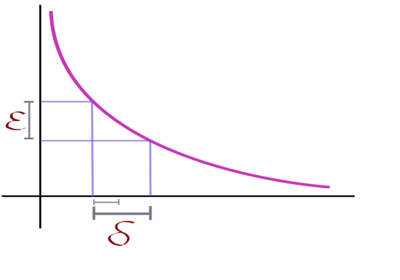
\includegraphics{./media/ComplexSeries/drawing3.png}
\caption{drawing3}
\end{figure}

So basically:

\begin{itemize}
\item
  A function is continuous if a \(\delta\)-value always exists and can
  be described as a function:

  \begin{itemize}
  \item
    \(\delta = \delta\left( \varepsilon, x \right) \)
  \end{itemize}
\item
  A function is uniformly continuous if a \(\delta\)-value always exists
  and can be described as a function only of \(\varepsilon\) :

  \begin{itemize}
  \item
    \(\delta = \delta\left( \varepsilon \right) \)
  \end{itemize}
\end{itemize}

\hypertarget{cantors-theorem}{%
\subsubsection{Cantor's Theorem}\label{cantors-theorem}}

If a function is continuous on an interval \(\left[ a,b \right] \), it
is uniformly continuous on that interval.

\begin{itemize}

\item
  The reasoning being that basically you could chose the smallest
  \(\delta\)-value that will work at all points on that interval
\end{itemize}

\hypertarget{why-is-uniform-continuity-important}{%
\subsubsection{Why is uniform continuity
important?}\label{why-is-uniform-continuity-important}}

Something like,

\begin{itemize}

\item
  if \(f\left( x \right) \) is uniformly continuous
\item
  Then: \[
  \int^{}_{} \lim_{}\left[ f\left( x \right)  \right]   \operatorname{d}x \iff \lim_{}\left[ \int^{}_{} f\left( x \right)   \operatorname{d}x  \right]
  \] but I'm not sure about this so don't quote me, we don't do it here
  so don't worry about it too much, we just need to show that we
  understand it the idea of uniformly continuous functions.
\end{itemize}

\hypertarget{problem-example}{%
\paragraph{Problem Example}\label{problem-example}}

\begin{quote}
Prove that the function \(f\left( x \right) = \frac{1}{1+ x^3}\) is
uniformly continuous on the interval \([1, \infty)\)
\end{quote}

So the first thing to notice is that \emph{Cantor's Theorem} cannot be
applied because it is an open interval.

\textbf{\emph{State the Definition}} \(f\left( x \right)\) is uniformly
convergent if:

\begin{align*}
  \forall x,y \in [1, \infty), \enspace \forall \varepsilon>0,& \enspace \exists \delta\left( \varepsilon \right) :\\
  &0<    \left| x- y \right| <\delta  \implies      \left| f\left( x \right) - f\left( y \right)  \right| < \varepsilon
\end{align*}

 \textbf{\emph{Work Backwards from the \(\varepsilon\) Definition}}

\begin{align*}
  \left| f\left( x \right) - f\left( y \right)  \right| &=     \left| \frac{1}{1+ x^3} - \frac{1}{1+ y^3}\right| \\
  &= \frac{    \left| y^3- x^3 \right| }{    \left| 1+ x^3 \right| \times     \left| 1+ y^3 \right| }\\
  &\leq \frac{    \left| y^3- x^3 \right| }{    \left| 1+ x^3 \right| }\\
  &= \frac{    \left| y- x \right| \cdot     \left| y^2+ xy+ x^2 \right| }{    \left| 1+ x^3 \right| }\\
  \text{Without loss of generality assume that $y<x$}\\
  &\leq     \left| y- x \right| \times 3\cdot \frac{    \left| x^2 \right| }{    \left| 1+ x^3 \right| }\\
  \text{Recall that $x\geq 1  \implies  \frac{1}{    \left| 1+ x^3 \right| }< \frac{1}{    \left| x \right| ^3}$}\\
  &\leq     \left| y- x \right| \cdot \frac{1}{    \left| x \right| } \cdot 3\\
  &\leq     \left| y- x \right| \cdot 3\\
  &\leq     3\cdot \delta\\
\end{align*}

 So choose \(\delta\):
\begin{align*}
3\delta &\leq \varepsilon\\
\delta &\leq \frac{\varepsilon}{3}
\end{align*}

\(\therefore\) it is sufficient to choose
\(\delta\leq \frac{\varepsilon}{3}\).

\textbf{\emph{Proof}}
\begin{align*}
  \forall x,y \in [1,\infty), \enspace \forall \varepsilon>0,& \enspace \exists \delta \leq \frac{\varepsilon}{3}
\end{align*}

\begin{align*}
  \left| x- y \right| < \delta  \implies      \left| f\left( x \right) - f\left( y \right)  \right| &\leq     \left| \frac{1}{1+ x^3} - \frac{1}{1+ y^3} \right| \\
  &\leq     \left| y- x  \right| \cdot \left( \frac{    \left| y^2 \right| +     \left| xy \right| +     \left| x^2 \right| }{    \left| 1+ x^3 \right| \cdot     \left| 1+ y^3 \right| } \right) \\
  &\leq     \left| y- x \right| \cdot \left( \frac{y^2}{    \left| 1+ y^3 \right| } +  \frac{    \left| x \right| \cdot     \left| y \right| }{    \left| 1+ x^3 \right| \cdot 1+ y^3} +  \frac{    \left| x^2 \right| }{    \left| 1+ x^3 \right| } \right) \\
  &leq     \left| y- x \right| \cdot \left( \frac{    \left| y \right| ^2}{    \left| y^3 \right| } +  \frac{    \left| x \right| \cdot     \left| y \right| }{    \left| x \right| ^3\cdot     \left| y \right| ^3} +  \frac{    \left| x \right| ^2}{    \left| x \right| ^3} \right) \\
  &\leq     \left| y- x \right| \cdot \left( \frac{1}{    \left| y \right| } + \frac{1}{    \left| x \right| \cdot     \left| y \right| }+ \frac{1}{    \left| x \right| } \right) \\
  &\leq     \left| y- x \right| \cdot \left(\frac{1}{1}+ \frac{1}{1\times 1}+ \frac{1}{1} \right) \\
  &\leq     \left| y- x \right| \cdot 3\\
  &< 3\cdot \delta\\
  &<3\times \frac{\varepsilon}{3}\\
&<\varepsilon\\
\square
\end{align*}

\end{document}
